
\section{Turing Machines and Complexity Measures}

A Turing machine is a theoretical device that implements a model of computation.
It operates on a tape of infinite length, which is divided into cells, and can
read and write symbols from/to each cell when the \textit{head} of the machine
is positioned over the cell. The Turing machine also has internal state, which
is finite and determines what actions it takes (reading, writing, moving the
tape etc).

In this course, we will be thinking about multi-tape Turing machines. Here, the
there are many tapes, numbered $1 \dots K$. Tape $1$ is the input tape and tape
$K$ is the output tape. The tapes inbetween the input and output tapes are the
work tapes. Any algorithm can be expressed as a multi-tape Turing machine

\subsection{Formally defining a Turing Machine}

A TM (Turing Machine) can be define as a quintuple, as shown in
Figure~\ref{fig:tm-definition}.

\begin{figure}[H]
  \centering
  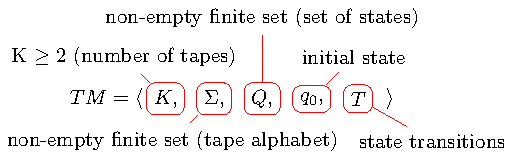
\includegraphics{equations/tm-definition}
  \caption{Part of a multi-tape Turing machine definition. We must also define
  the word \textit{symbol}, which is a mark occupying one cell on the tape. The
  alphabet that a symbol can be from is $\Sigma \cup \{
  \textrm{\textvisiblespace}, \vartriangleright\}$, where \textvisiblespace~is a
  blank cell, and $\vartriangleright$ is the start symbol (signifying the left
  edge of the tape).}
  \label{fig:tm-definition}
\end{figure}

Up to now, we've defined a TM that is perfectly formed\dots but does nothing. We
need to define how it moves between states in $Q$. To do that, we define a
transition, as in Figure~\ref{fig:tm-transition}.

\begin{figure}[H]
  \centering
  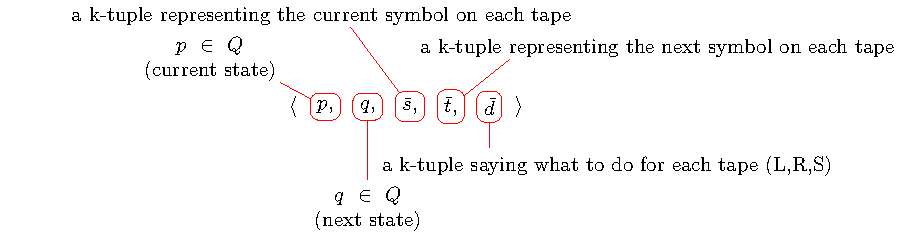
\includegraphics{equations/tm-transition}
  \caption{A transition of a Turing Machine}
  \label{fig:tm-transition}
\end{figure}

Informally, this transition applies only if the current state is $p$, and the
squares on the tapes confirm to $\bar{s}$, then set the new state to $q$ and
write the symbols from $\bar{t}$ to the tapes and move the heads as directed by
$\bar{d}$ (Left, Right or Stay).

Now we've nearly finished defining a multi-tape TM, the final points are:

\begin{itemize}
  \item Since the TM is deterministic, there can be \textit{at most} one 
    transition for every $(state,~\overline{\text{\textit{current symbols}}})$ 
    tuple.
  \item The tape never moves left past the $\vartriangleright$ symbol.
  \item Tape 1 is read only and tape $K$ is write only.
\end{itemize}

\subsubsection{Acceptance, computability and recognisability}

We say that a TM $M$ \textit{accepts} an input $x$ if it halts on $x$. The
language \textit{recognised} by $M$ is the set of strings that is accepted by
$M$.

\marginpar{Remember, when we say `Turing Machine', we could mean either a 
deterministic TM or a non-deterministic one (unless we explicitly said which one
we meant of course!).}

If a language is recognised by a nondeterministic Turing Machine $M$, then there
is also a  deterministic Turing Machine $M'$ that will recognise the same
language.

A language is \textit{computable} (aka decidable), if there is a (deterministic)
TM that will accept every string in the language, and reject every string not in
the language.

Up to now, our definitions of recognisable and computable are pretty similar (if
not the same). The difference is, that if an input string \textbf{isn't} in a
computable language, then the TM will halt (and output `no'), whereas if the
input string isn't in a recognisable language, then the TM \textit{may} halt and
output `no', or it could just carry on computing for ever. All a Turing Machine
does with a recognisable language, is recognise if a string is in the language,
it makes no guarantees about string not in the language!

\subsubsection{Nailing that TM definition}

If you want your Turing Machines very well defined, then this how you do it
(alternately, read Chapter 3 of Sipser).

%TODO: Not sure about a configuration on slide 8 of lecture 7b. I emailed Ian.

A run of a TM is terminating if it is finite. If the input to a deterministic TM
$M$ is $x$, and the run is finite, we write $M \downarrow x$ otherwise, if the
run is infinite, we write $M \uparrow x$.

Let $M$ be a deterministic TM over the alphabet $\Sigma$, and its input be $x
\in \Sigma^*$ (i.e. the input is zero or more symbols from the alphabet). If $M
\downarrow x$ then the output tape of $M$ will contain some string $y \in
\Sigma^*$ once M has finished computing. The cool thing, is that we can treat
$M$ like a function, lets call it $f_M$, that operates over $\Sigma^*
\rightarrow \Sigma^*$:

\[
  f_M(x) = \begin{cases}
       y & if M \downarrow x\\
       \text{undefined} & if M \uparrow x\\
     \end{cases}
\]

In this case, $M$ computes the function $f_M$.

\subsubsection{The Universal Machine}

If you're that way inclined, you can do lots of cool things with Turing
Machines. One such cool thing, is that every TM is a finite thing (it's just a
quintuple as shown in Figure~\ref{fig:tm-definition}), which means we can come
up with a way of encoding any Turing Machine into a string over the alphabet
$\Sigma$ and use it as input to another Turing Machine!

If we can do this, then we can construct a \textbf{Universal Machine} $U$. This
machine takes two `arguments', another TM $M$ (encoded of course) and some
arbitrary input $x$. If $M \downarrow x$, then $U$ finishes with $y$ on its
output tape. If $M \uparrow x$, then $U$ will never terminate. The input is
coded as $M;x$, where `;' is a separator between the Turing Machine we're
`simulating' and the input we'll give it.

\subsubsection{Enumerators}

Enumerators aren't in the course slides, but they do appear in the reading. Skip
this section if you're doing last minute cramming.

An Enumerator is a Turing Machine with an attached printer. Now, I know what
you're thinking; \textit{I'm a computer scientist, I hate printers. Why would
anybody combine a complicated enough idea like a TM with a printer?!}
Enumerators have an important theoretical use though, and don't require us to
install drivers like we do for printers, and they certainly don't need to work
over WiFi (so this section should be a piece of cake really).

The TM inside an enumerator is able to send a string to the printer whenever it
wants to print out a string. If the TM does not halt, then the printer may print
an infinite list of strings. The language that is \textit{enumerated} by the
enumerator, is the collection of strings that it eventually prints out. Since
there are no rules about repetitions or ordering in the output list of the
printer, you might want to think about the enumerated language as a set.

So, as I said before, enumerators \textit{are} useful. Namely a language is
Turing recognisable if and only if, there is some enumerator that enumerates it.

Its easy to show that a TM can recognise a language that is enumerated by an
enumerator, just build a TM that does this:

\begin{enumerate}
  \item We have an input word $w$
  \item Run the enumerator $E$:
  \begin{enumerate}
    \item Every time $E$ outputs a new string, compare it to the word $w$
    \item If they are equal, then accept the word.
  \end{enumerate}
\end{enumerate}

Note that there is the potential for this TM to run for an infinite length of
time, if the enumerator generates an infinite list, and $w$ is not in the
language it enumerates.

We can also make an enumerator enumerate any language that is recognised by a
Turing Machine $M$:

\begin{enumerate}
  \item Ignore any input
  \item For $i = 1$ to $i = \infty$
  \begin{enumerate}
    \item Run the TM $M$ for $i$ steps for all possible strings of length $i$ in
      the language ($\Sigma^i$)
    \item If any computations accept, then print out the corresponding string.
  \end{enumerate}
\end{enumerate}

This enumerator will never halt (since it loops infinitely many times over an
infinitely large set of input strings), but eventually, it will print out all of
the words in the language (even though there will be \textit{a lot} of
duplicates!).

\subsection{The Halting problem}

The Halting problem asks:

\begin{quote}
  Given a Turing Machine $M$ and a string for its input $x$, return:
  \begin{itemize}
    \item[] \textbf{Yes} if $M \downarrow x$ ($M$ decides $x$)
    \item[] \textbf{No} otherwise, where $M$ would compute forever
  \end{itemize}
\end{quote}

Turing managed to prove that there is no Turing Machine that will decide the
Halting problem. The proof is fairly simple, but it takes a while to get your
head around it when its written in a mathematical form. Luckily, I found a poem,
written in the style of \href{https://en.wikipedia.org/wiki/Dr._Seuss}{Dr.
Seuss}, that provides a better textual explanation than I ever could; see
Figure~\ref{fig:halting-poem}.

\begin{figure}[h]
\begin{minipage}{\textwidth}
  \newgeometry{top=2cm,bottom=2cm,left=1cm,right=3cm}
  \begin{mymulticols}
  \poemtitle{Scooping the Loop Snooper\newline{\small An elementary proof of the 
  undecidability of the halting problem}}
\settowidth{\versewidth}{And this program called Q wouldn't stay on the shelf;}
\begin{verse}[\versewidth]
  No program can say what another will do.\\
  Now, I won't just assert that, I'll prove it to you:\\
  I will prove that although you might work til you drop,\\
  you can't predict whether a program will stop.

  Imagine we have a procedure called P\\
  that will snoop in the source code of programs to see\\
  there aren't infinite loops that go round and around;\\
  and P prints the word “Fine!” if no looping is found.

  You feed in your code, and the input it needs,\\
  and then P takes them both and it studies and reads\\
  and computes whether things will all end as they should\\
  (as opposed to going loopy the way that they could).

  Well, the truth is that P cannot possibly be,\\
  because if you wrote it and gave it to me,\\
  I could use it to set up a logical bind\\
  that would shatter your reason and scramble your mind.

  Here's the trick I would use - and it's simple to do.\\
  I'd define a procedure - we'll name the thing Q -\\
  that would take any program and call P (of course!)\\
  to tell if it looped, by reading the source;

  And if so, Q would simply print “Loop!” and then stop;\\
  but if no, Q would go right back to the top, \\
  and start off again, looping endlessly back,\\
  til the universe dies and is frozen and black.

  And this program called Q wouldn't stay on the shelf;\\
  I would run it, and (fiendishly) feed it itself.\\
  What behaviour results when I do this with Q?\\
  When it reads its own source, just what will it do?

  If P warns of loops, Q will print “Loop!” and quit;\\
  yet P is supposed to speak truly of it.\\
  So if Q's going to quit, then P should say, “Fine!” -\\
  which will make Q go back to its very first line!

  No matter what P would have done, Q will scoop it:\\
  Q uses P's output to make P look stupid.\\
  If P gets things right then it lies in its tooth;\\
  and if it speaks falsely, it's telling the truth!

  I've created a paradox, neat as can be -\\
  and simply by using your putative P.\\
  When you assumed P you stepped into a snare;\\
  Your assumptions have led you right into my lair.

  So, how to escape from this logical mess?\\
  I don't have to tell you; I'm sure you can guess.\\
  By reductio, there cannot possibly be\\
  a procedure that acts like the mythical P.

  You can never discover mechanical means\\
  for predicting the acts of computing machines.\\
  It's something that cannot be done. So we users\\
  must find our own bugs; our computers are losers!
\end{verse}
\attrib{Geoffrey~K.~Pullum, Scooping the loop snooper: An elementary proof of
the undecidability of the halting problem. Mathematics Magazine 73.4 (October
2000), 319-320}
  \end{mymulticols}
  \restoregeometry
\end{minipage}
\caption{A poetic explanation of the Halting Problem.}
\label{fig:halting-poem}
\end{figure}

As nice as it is, I think it's unlikely that the poem would be accepted as an
answer in an exam, so we'd better learn the formal definition of the Halting
problem too.

Suppose we have a TM $P$ that can determine if another TM can halt. We're going
to make another TM $Q$ that is defined so:

\begin{enumerate}
  \item Duplicate the input $x$ TM we're given.
  \item Run $P$ on the duplicated input ($x;x$).
  \begin{itemize}
    \item[] $P(x;x) = Y$, then Loop 
    \item[] $P(x;x) = N$, then Halt
  \end{itemize}
\end{enumerate}

Now, if we give $Q$ the input $Q$, then the embedded $P$ will receive $(Q;Q)$,
meaning that if:

\begin{description}
  \item $Q \downarrow Q \implies Q \uparrow Q$
  \item $Q \uparrow Q \implies Q \downarrow Q$
\end{description}

% TODO: Find another explination of the halting problem

\subsection{Complexity}

You already know that there are two types of Turing Machine; deterministic and
non-deterministic TM's, but now its time to think about the resources that
Turing Machines consume. We don't think of TM resources as commodities such as
metal, electricity etc, since TM's are abstract, theoretical devices. Instead
the two commodities we're interested in with Turing Machines are \textbf{time}
and \textbf{space}.

If we have a TM $M$, and let $g : \mathbb{N} \rightarrow \mathbb{N}$. $M$ runs
in time $g$ if for any finite input $x$, $M$ takes at most $g(|x|)$ steps. We
say that $M$ runs in space $g$ if for any finite $x$, $M$ takes at most $g(|x|)$
squares on its tapes.

If you think about it, this is nearly a formal way of defining the Big-Oh
notation. One of the main problems with this, is that TM's might execute at
different speeds (maybe one has faster motors for its tape etc). This means that
the algorithms we're designing will have certain runtimes on certain machines.
In order to mitigate this, we like to define sets of functions for the Big-Oh
notation; $M$ runs in time $G$ if for some $g \in G$, $M$ runs in time $g$.

This means that the Big-Oh notation can ignore things like constants, and lets
us abstract away the details of Turing machines (like exactly how many
operations it takes to multiply two numbers).

In fact, possibly the simplest definition of complexity is to let $L$ be a
language, and $G$ be a set of functions from $\mathbb{N}$ to $\mathbb{N}$. $L$
is in \texttt{TIME/SPACE(G)} if there exists a deterministic TM that decides
$L$ in time/space G.

Similarly, if we can find a non-deterministic TM to recognise $L$, then we say
that $L$ is in \texttt{NTIME/NSPACE\{G\}}.

\subsubsection{Complexity classes}

As you probably know, there are several different complexity classes, as shown
in Table~\ref{tbl:complex-classes}.

\marginpar{Note, you can't have $Time(log(n))$ since reading the input takes
$n$ time.}

\begin{table}[h]
  \begin{tabular}{l >{$}l<{$} l >{$}l<{$}}
    & & LogSpace & Space(log(n))\\
    PTime & Time(n) & PSpace & Space(n)\\
    ExpTime & Time(2^{n}) & ExpSpace & Space(2^{n})\\
    k-ExpTime & Time(2^{2^{\dots^2\}^{n} \leftarrow k~times}}) & 
      k-ExpSpace & Space(2^{2^{\dots^2\}^{n} \leftarrow k~times}})\\
  \end{tabular}
  \caption{The deterministic complexity classes}
  \label{tbl:complex-classes}
\end{table}

To get their non-deterministic counterparts, just stick an `N' on the front of
everything, as in Table~\ref{tbl:complex-classes-nondet}.

\begin{table}[h]
  \begin{tabular}{l >{$}l<{$} l >{$}l<{$}}
    & & NLogSpace & NSpace(log(n))\\
    NPTime & NTime(n) & NPSpace & NSpace(n)\\
    NExpTime & NTime(2^{n}) & NExpSpace & NSpace(2^{n})\\
    Nk-ExpTime & NTime(2^{2^{\dots^2\}^{n} \leftarrow k~times}}) & 
      Nk-ExpSpace & NSpace(2^{2^{\dots^2\}^{n} \leftarrow k~times}})\\
  \end{tabular}
  \caption{The deterministic complexity classes}
  \label{tbl:complex-classes-nondet}
\end{table}

Obviously, some complexity classes can fit inside each other. Here are some
examples:

\[
  PTime \subseteq ExpTime \subseteq 2-ExpTime \subseteq \dots
\]

\[
  LogSpace \subseteq PSpace \subseteq ExpSpace \subseteq \dots
\]

\[
  NPTime \subseteq NExpTime \subseteq N2-ExpTime \subseteq \dots
\]

We can also interleave the non-deterministic classes:

\[
  PTime \subseteq NPTime \subseteq ExpTime \subseteq NExpTime \subseteq \dots
\]

Finally, the $Co^*$ complexity classes are the ones that describe the
complementary languages to those described by the others. For example, if we can
decide a language $L$ over $\Sigma^*$ in \texttt{NPTime}, then we can decide
$\Sigma^* - L$ in \texttt{Co-NPTime}. We know that \texttt{Time(G) =
Co-Time(G)}, and the same for space, but not if \texttt{NPTime(G) = Co-NPTime}.
